
\documentclass[aps,twocolumn,secnumarabic,nobalancelastpage,amsmath,amssymb,
nofootinbib]{revtex4}

% nofootinbib is another document class option that allows you to put
% footnotes on the page where they occur rather than at the end of the
% paper.  This makes for easier reading!

% secnumarabic is a particularly nice way of identifying sections by
% number to aid electronic review and commentary.

% amsmath and amssymb are necessary for the subequations environment
% among others

\usepackage{chapterbib}
\usepackage{color}
\usepackage{graphics}      % standard graphics specifications
\usepackage{graphicx}      % alternative graphics specifications
\usepackage{longtable}     % helps with long table options
%\usepackage{url}          % for on-line citations (conflicts with hyperref)
\usepackage{bm}            % special 'bold-math' package
\usepackage[colorlinks=true]{hyperref}


\begin{document}
\title{Sample Report}
\author         {Adnan Basar (Partner: Kadir Simsek)}
\email          {adnanbasarr@icloud.com}
\affiliation    {2010205108}
\date{\today}





\begin{abstract}
Aim
\end{abstract}

\maketitle

%%%%%%%%%%%%%%%%%%%%%%%%%%%%%%%%%%%%%%%%%%%%%%%%%%%%%%%%%%%%%%%%%%
\section{Introduction}



\section{Experimental Setup}

Light comes in discrete packets, called $photons$, each with an energy proportional to its frequency.  
\begin{align}
E = h\nu
\end{align}

For each metal, there exists a minimum binding energy for an electron characteristic of the element, also called the work function ($W_0$).  When a photon strikes a bound electron, it transfers its energy to the electron.  If this energy is less than the metal's work function, the photon is re-emitted and no electrons are liberated.  If this energy is greater than an electron's binding energy, the electron escapes from the metal with a kinetic energy equal to the difference between the photon's original energy and the electron's binding energy (by conservation of energy).  Therefore, the maximum kinetic energy of any liberated electron is equal to the energy of the photon less the minimum binding energy (the work function).  Expressed concisely the relationship is as such:
\begin{align}
\label{eq:kmax}
K_{max} = h\nu - W_0
\end{align}

This maximum kinetic energy can be determined by applying a retarding potential ($V_r$) across a vacuum gap in a circuit with an amp meter.  On one side of this gap is the photoelectron emitter, a metal with work function $W_0$.  We let light of different frequencies strike this emitter.  When $eV_r = K_{max}$ we will cease to see any current through the circuit.  By finding this voltage we calculate the maximum kinetic energy of the electrons emitted as a function of radiation frequency.  This relationship (with some variation due to error) should model Equation \ref{eq:kmax} above.

\section{Data Analysis}

\subsection{Schematic}

adann

\begin{figure}[htbp]
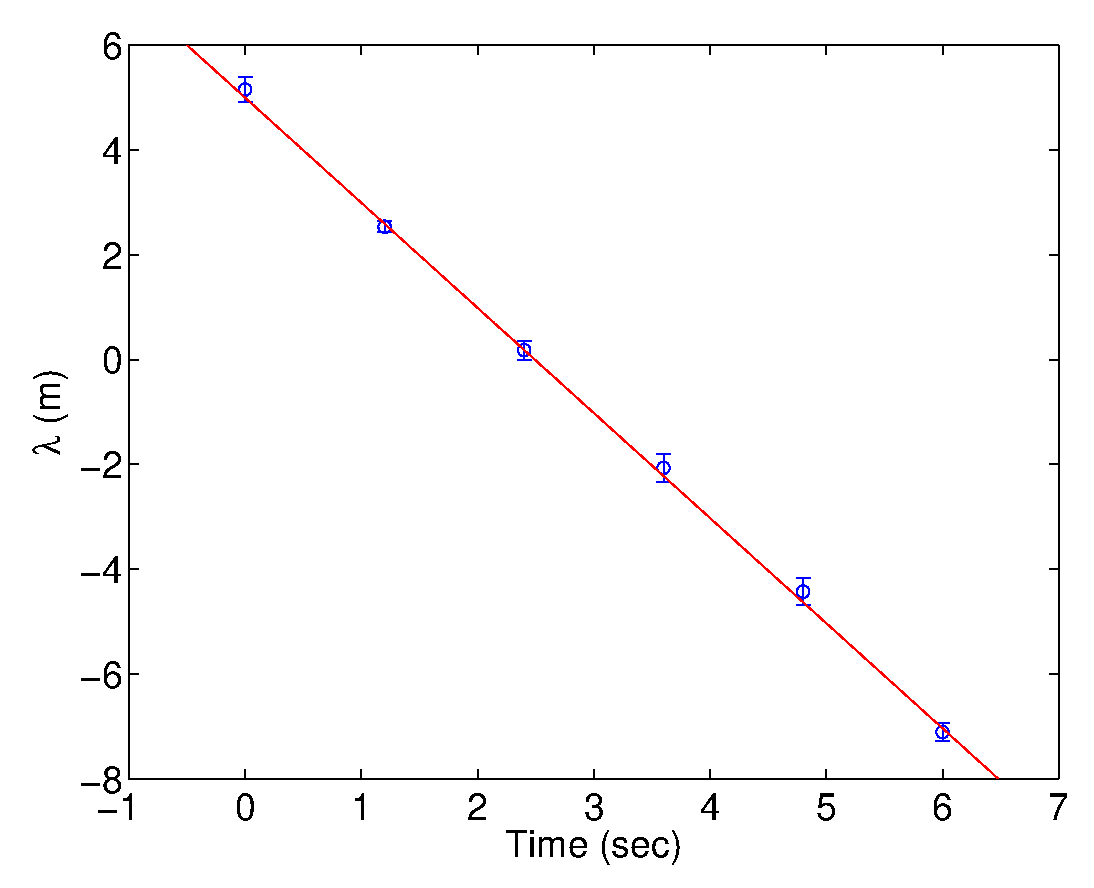
\includegraphics[width=2.5in]{schematic}
\caption{Schematic of experimental setup with retarding voltage applied.  Photons are incident on the photocathode and travel toward the anode to complete the circuit unless stopped by a high enough applied voltage.}
\label{fig:schematic}
\end{figure}

\subsection{Apparatus}

Our monochromatic light source was an Oriel 65130 Mercury Lamp in combination with a narrow band pass filter wheel with four different wavelength passbands.  The wavelengths are listed in Table \ref{tab:wavelengths}.

\begin{center}
\begin{table}[htbp]
\begin{tabular}{|c|}
\hline
Wavelengths (nm)\\
\hline
365.0 $\pm$ 2.0 \\
404.7 $\pm$ 2.0 \\
546.1 $\pm$ 2.0 \\
577.0 $\pm$ 2.0\\
\hline
\end{tabular}
\caption{\label{tab:wavelengths}Spectrum from Oriel mercury lamp.}
\end{table}
\end{center}
A Leybold photocell served as our target, containing a potassium ($W_0 = 2.3 eV$) photosurface as the cathode and a platinum ring ($W_a = 5.7 eV$) as the anode separated by a vacuum.  It was enclosed in a black box with a small circular opening to allow for incoming light.  Precautions were taken to shield the setup from ambient light, to protect the filters and photocell from overheating, and to minimize illumination of the anode.


\section{Data and Analysis}

An example of our tabulated raw data is shown in Table \ref{tab:raw} for the 365.0 nm wavelength over five trials.  




The normalized currents for each wavelength are plotted against their respective retarding voltages in Figure \ref{fig:normcurrent} with the standard deviations as error bars.  The normalization removes the scaling effects of the non-uniform distribution of intensities across the spectrum of our light source.  With intensity normalized away, it is already evident from this figure that the cut-off voltages have some dependence on frequency.

\begin{figure}[htbp]
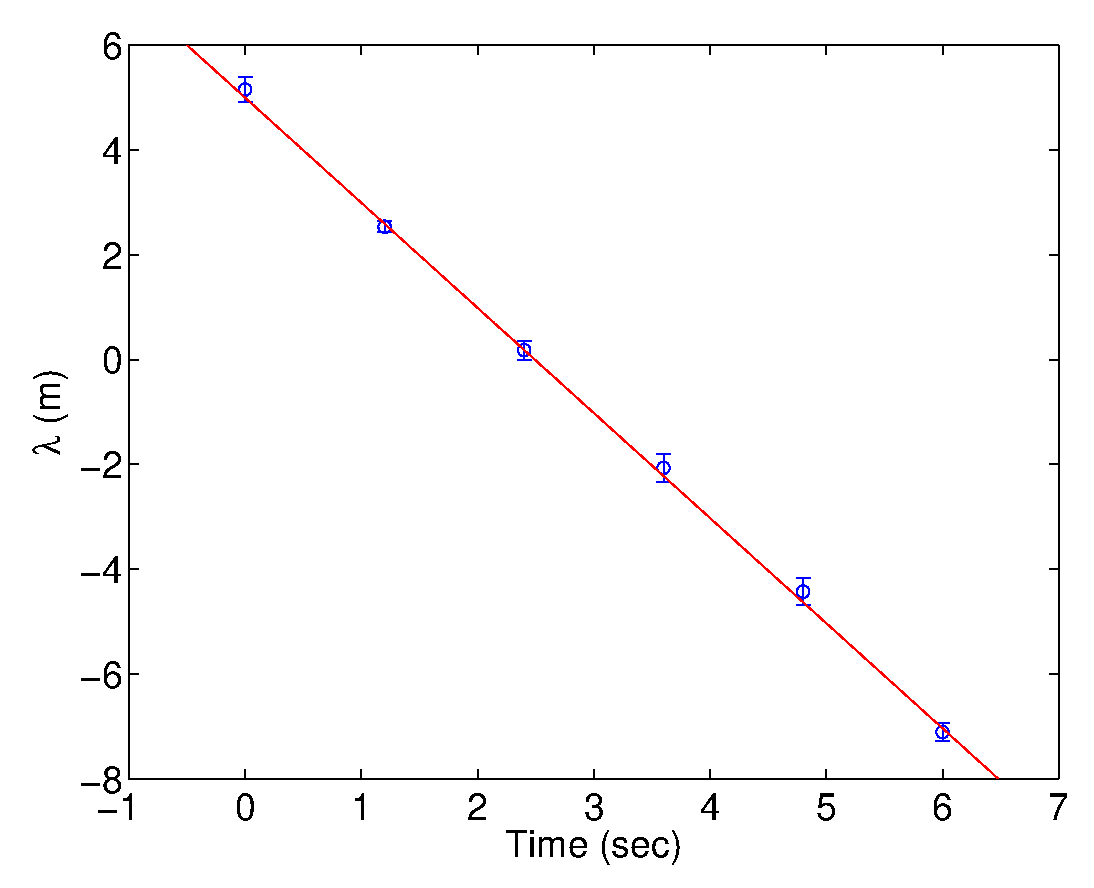
\includegraphics[width=3.5in]{graph_norm}
\caption{\label{fig:normcurrent}Plot of photocurrent as a function of the magnitude of retarding voltage applied for each wavelength of incident light.  Normalized to the zero-voltage point of the lowest intensity wavelength.}
\end{figure}

A back current was a noticeable effect for several wavelengths.  Back current is caused by photoelectrons liberated from the platinum anode as a result of scattered light.  Its effects become most prominent when the retarding voltage is high.  The retarding voltage is seen as an accelerating voltage by these electrons and they travel uninhibited from the anode to the cathode, opposite the direction of the expected flow. 

Another feature that should not be neglected is the non-linear nature of the photocurrent vs. voltage curve near the stopping voltage.  Theoretically, at the stopping voltage, we expect the current to be zero.  However, as we decrease the stopping voltage, the current rises only very slowly until it begins to take on a familiar $I = \alpha V_r$ linear form.  This is to be expected since the number of states with energy near the minimum binding energy $N(E\approx-W_0)$ may in fact be very small, and increases as the binding energy increases.

Complicating effects such as the two represented above compromise the reliability of zero-current crossings for determination of stopping voltages.  Instead, we look to two different methods for extrapolating the data points of interest.  Any differences in results will be used in calculation of a lower bound on our systematic error.


\subsection{Method One for Voltage Cut-Off Determination: Linear Fit Method}



Since the asymptotic behavior of each curve at both low and high values of retarding voltages (discounting saturation) is linear, both sections can be fit to separate linear regressions.  The criteria for determining how many data points to fit on each end was simple: minimum number of points required for a meaningful fit while maintaining a reasonable $\chi^2$.  A linear fit should involve greater than two points but maintain a $\chi^2$ of less than 100.  Therefore three data points were chosen on each end of the data set for their respective regressions.

The intersection of these two theoretical fits is a point ($V_s,I_0$).  $V_s$ is an estimate for the stopping voltage extrapolated from the two linear relations and $I_0$ the baseline current.  Performing this analysis on all four sets of data, we obtain the results tabulated below:



\begin{center}
\begin{table}[htbp]
\begin{tabular}{|l|c|c|r|}
\hline
{\small Wavelength ($\lambda$)} & {\small St. Voltage ($V_s$)} & {\small Error ($\sigma_{V_s}$)} & {\small Relative Error} \\
\hline
365.0 nm & 0.76 V & 0.16 V & 21.6\% \\
404.7 nm & 0.60 V & 0.12 V & 20.1\% \\
546.1 nm & 0.44 V & 0.09 V & 20.2\% \\
577.0 nm & 0.44 V & 0.09 V & 20.3\% \\
\hline
\end{tabular}
\caption{\label{tab:linfitresults} Obtained by the Linear Fit Method, we find a linear dependence of stopping voltage values on wavelength of light.}
\end{table}
\end{center}


Since equation \ref{eq:kmax} can be written as,
\begin{align}
K_{max} = eV_s = h\nu - W_0,
\end{align}

We can divide by $e$ and rewrite the equation in units of electron-Volts (eV).
\begin{eqnarray}
\label{eq:main}
K_{max}[in ~eV] = V_s = (h/e)\nu - W_0 [in ~eV]
\end{eqnarray}



Figure \ref{fig:he} shows a plot of the maximum determined kinetic energy (in electron-Volts) of photoelectrons as a function of the frequency of light (in Hz).  The linear regression shows the best fit line through this set of reduced data points.  The slope of this line corresponds to the value of Planck's constant $h$ in $eV \cdot s$.

\vspace{0.3in}

\textbf{This method yields a value for $h$ of $(9.4 \pm 4.8) \times 10^{-16} ~eV\cdot s$.}

\subsection{Method Two for Voltage Cut-Off Determination: Zero-Slope Method}

Observing the qualitative character of the normalized currents vs. voltages graphs one can conceive of a slightly more direct way of accounting for the effects of back current.  If we treat (somewhat erroneously but reasonably) the back current as a constant negative offset on the curve in the high-voltage region of the data, where the current should be zero, we can extrapolate the stopping voltage to be the point at which the curve reaches a constant value and does not change for any larger magnitude applied voltage.

We call this method the Zero-Slope or Point-Deviation Method.  It reads the data points for each wavelength from right to left and picks out the first point that deviates from the flat-line end behavior and assigns that value to be the stopping voltage for that particular wavelength.  We tested the precision of this method by setting different threshold (minimum deviation) values and observing any change in resulting data set.  For a threshold between 0 and 0.5 this method yielded the exact same set of points and values.  Since this method relies on discrete points, the "real" value can fall anywhere between the chosen value and the next points on either end, so we estimated the error in stopping voltage to be about the interval between successive data points.




\textbf{Using this method of analysis, $h$ was determined to be $2.9 \times 10^{-15} \pm 7.7 \times 10^{-16} ~eV \cdot s$.}


\subsection{Combined Result}

\textbf{The combined result of the two analyses is an average $h$ value of $1.92 \times 10^{-15} ~eV \cdot s$ with a total error of $1.08 \times 10^{-15} ~eV \cdot s$}.  This will be derived and elaborated upon in the next section.

\section{Error Contributions and Calculations}

Incidentally, according to theory, the y-intercept of the relation defined by Equation \ref{eq:main} should correspond to the work function ($W_0$) of potassium (2.3 eV).  However, we see that this is not nearly the case.  More subtle forces are at play which contribute to the disparity between theoretical predictions and actual results.  

The applied voltage difference between the cathode and the anode metals is not the voltage difference that an electron "sees" as it is traveling between them.  Following the argument presented by Melissinos \cite{melissinos}, energy loss around a closed circuit loop must be zero with no dissipative elements.  Thus, the electron sees not the applied voltage V' but a voltage V adjusted by the work functions of the two metals.  An illustration (Figure \ref{fig:melissinos}) from the same source \cite{melissinos} pg. 20 helps facilitate the explanation.  


\begin{figure}[htbp]
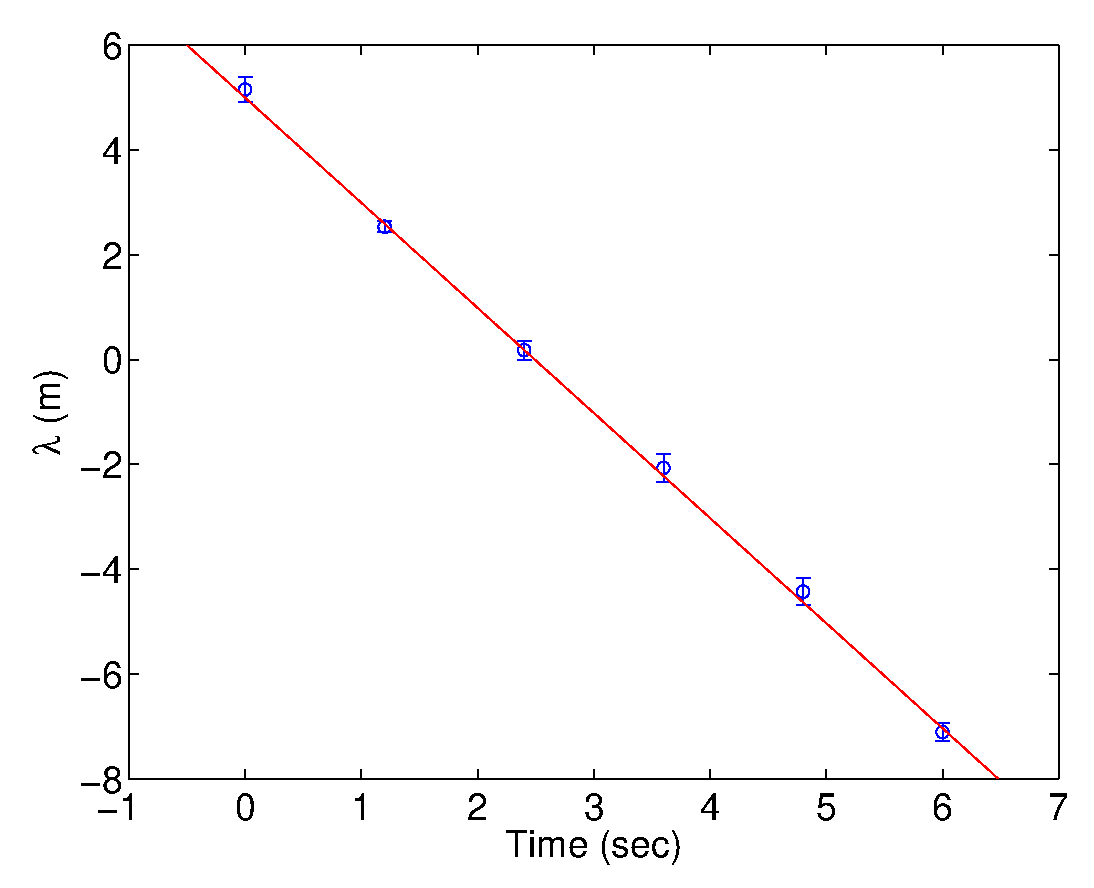
\includegraphics[width=2.2in]{melissinos}
\caption{\label{fig:melissinos} The actual voltage overcome by the electron in its journey is $V = V'-(\phi_a - \phi_c$).  Here, $\phi_a = W_a$ and $\phi_c = W_0$.}
\end{figure}

If we solve for the actual y-intercept in the relationship we find it to be the work function of the anode ($W_a$) instead of the cathode.  However, this is still not well-represented by the data.  If our objective was to obtain an accurate work function, we would need to change certain aspects of our experiment.  We would want to use purer metals as opposed to alloys.  Care must be taken to avoid cathode material deposition onto the anode.  Measurements should be extended until current saturation (the voltage becomes an accelerating voltage) so we can better define and correct for the back current effect.

In this case we're mostly interested in the slope of the relation between $K_{max}$ and $\nu$ for our value of $h/e$.  The two error contributions are systematic and random error.  The systematic error is set by the difference betweeen our two methods of evaluating the cut-off voltage while the random errors propagate through our analysis from their origins in the measurements we took.

The random error in our raw data is determined experimentally through five independent trials \footnote{These trials were assumed to be independent (measured from low voltage to high voltage each time) but in some cases did not match the statistical distribution for independent random error.} using the formula for the square-root of the variance, $\sigma_I$.
\begin{align}
\sigma_I^2 = \frac{1}{5} \sum_{i=1}^5 (I_i - \langle I \rangle)^2
\end{align}

Any linear regression $y=mx+b$ calculated from our input variables and errors outputs an uncertainty on $m$ and on $b$.  In the case of finding the intersection of two linear regression lines $y=m_1 x+b_1$ and $y = m_2 x + b_2$, the error propagation formula was used to derive the following result for error on the X-coordinate of the intersection point in 2-D space:
\begin{align} 
\nonumber \sigma_x^2 &= \left(\frac{1}{m_1 - m_2}\right)^2 \sigma_{b_2}^2 + 
             \left(\frac{1}{m_1 - m_2}\right)^2 \sigma_{b_1}^2 \\ &+
		 \left(\frac{b_2 - b_1}{(m_1 - m_2)^2}\right)^2 \sigma_{m_1}^2 +
		 \left(\frac{b_2 - b_1}{(m_1 - m_2)^2}\right)^2 \sigma_{m_2}^2
\end{align}

When faced with two different calculated values for Planck's constant ($h_1$ and $h_2$), and their respective uncertainties ($\sigma_{h_1}$ and $\sigma_{h_2}$), we determined our final value of $h$ by taking the average, 
\begin{align}
h = \bar{h} = \frac{h_1 + h_2}{2} = 1.92 \times 10^{-15} eV \cdot s
\end{align}

and determined our random error on $h$, $\sigma_{h_r}$, by propagating both uncertainties using the formula,
\begin{align}
\sigma_{h_r}^2 = \frac{1}{4} \sigma_{h_1}^2 +  \frac{1}{4} \sigma_{h_2}^2 = 2.12 \times 10^{-31} eV^2 s^2.
\end{align}

The systematic error was estimated by the square-root of the variance of $h_1$ and $h_2$ and determined to be $9.8 \times 10^{-16} ~eV \cdot s$.

The total error on $h$ is a combination of random error ($\sigma_{h_r}$) and systematic error ($\sigma_{h_s}$), 
\begin{align}
&\sigma_{h}^2 = \sigma_{h_s}^2 + \sigma_{h_r}^2 \\ \nonumber
&\sigma_{h} = 1.08 \times 10^{-15} ~eV \cdot s
\end{align}


\section{Conclusions}

Our experiment verified our hypothesis.  We observed light behave as if it were a particle (not a wave) in its interaction with matter.  We were able to demonstrate for light the linear dependence of its energy on its wavelength and determine to some accuracy the constant of proportionality.  The actual value of Planck's constant fell outside of our errorbars, which is less than ideal.  Our final uncertainty on the value proved to be 50\% of the value itself.  This is very large and makes the task of drawing solid conclusions difficult.  

Though we cannot necessarily reduce random errors, we can seek to better characterize it in our experiments.  This can be accomplished through not only more repeated trials but especially more independent trials.  If, in the future, we attempt to reset the amp meter and voltage supply for each trial or wait a longer period of time between trials, we may find a more representative variance in our measurements.

There are means, however, of reducing our systematic error.  In addition to the changes and improvements suggested previously at the end of the discussion on work functions, by simply taking more data points and extending our observations deeper into the high and low voltage ends, we avail ourselves of more discriminating information to adjust for our systematic error.  Furthermore, the usage of a brighter source can offer us more resolution on our curves and allow us to better identify a cut-off voltage.

There are extensions on our experiment that may and should be explored in the future.  Changing other variables, including intensity and the cathode/anode work function and observing its effects on the system, may provide us with further and confirming evidence on the particle nature of light.

\bibliography{photoelectric}


%%%%%%%%%%%%%%%%%%%%%%%%%%%%%%%%%%%%%%%%%%%%%%%%%%%%%%%%%%%%%%%%%%%%%%%%%%%%%
\begin{acknowledgments} We are grateful of the assistance we received from the Junior Lab TA's and Professor with this experiment.

All linear regressions were calculated using the fitlin.m MATLAB program offered on the Junior Lab website http://web.mit.edu/8.13/www/jlmatlab.shtml.
\end{acknowledgments}

%%%%%%%%%%%%%%%%%%%%%%%%%%%%%%%%%%%%%%%%%%%%%%%%%%%%%%%%%%%%%%%%%%%%%%%%%%%%%

\end{document}
